\documentclass{article}
\usepackage[a4paper, left=2cm, right=2cm, top=1.5cm, bottom=1.5cm]{geometry}
\usepackage[heading=true, zihao=-4, UTF8]{ctex}
\usepackage{setspace}
\usepackage{graphicx}     %插入图片的宏包
\usepackage{float}        %设置图片浮动位置的宏包
\usepackage{abstract}     %设置摘要样式
\usepackage{caption}      %标签
\usepackage{booktabs}
\usepackage{multirow} % 用于合并单元格(可选)
\usepackage{fontspec}   %设置英文字体
\usepackage{titletoc}     %设置目录样式
\usepackage{amsmath}

\setmainfont{Times New Roman} %设置英文字体

\let\kaishu\relax
\newCJKfontfamily\kaishu{KaiTi}[AutoFakeBold]
\let\songti\relax
\newCJKfontfamily\songti{SimSun}[AutoFakeBold]

\ctexset{
  section = {
    format += \zihao{3} \heiti \mdseries,
    aftername = \hspace{0.5em}
  },
  subsection = {
    format += \zihao{-3} \heiti \mdseries,
    aftername = \hspace{0.5em}
  } ,
  subsubsection = {
    format += \zihao{4} \heiti \mdseries,
    aftername = \hspace{0.5em}
  }
}

\renewcommand{\contentsname}{\zihao{3}\heiti\mdseries 目\ \ \ 录}
\titlecontents{section}[0pt]{\vspace{0.25\baselineskip} \mdseries \zihao{-4}}{\contentslabel{1em}}{}{\titlerule*[0.25pc]{.} \contentspage}
\titlecontents{subsection}[2.6em]{\vspace{0.25\baselineskip} \mdseries \zihao{-4}}{\contentslabel{1.6em}}{}{\titlerule*[0.25pc]{.} \contentspage}
\titlecontents{subsubsection}[4.3em]{\vspace{0.25\baselineskip} \mdseries \zihao{-4}}{\contentslabel{2.3em}}{}{\titlerule*[0.25pc]{.} \contentspage}

\renewcommand {\thetable} {\thesection{}-\arabic{table}}    %设置表格编号与章节对应
\renewcommand {\thefigure} {\thesection{}-\arabic{figure}}  %设置图片编号与章节对应
\numberwithin {equation}{section}

\captionsetup {
  font={
    small,
    stretch=1.25
  },
  labelsep=space
}

\begin{document}
\zihao{-4}

\pagestyle{empty} %自定义封面
\begin{center}
  {\zihao{-4} \hspace{1em} \\ \vspace{1em}}
  {\zihao{0} \songti 珠海科技学院 \\ \vspace{1em}}
  {\zihao{0} \songti \textbf{毕\ 业\ 设 \ 计} \\ \vspace{1em}}
  {\zihao{-1} \kaishu \textbf{基于FPGA的JPEG图像编解码系统设计} \\ \vspace{4em}}
  \zihao{-2}
  \kaishu
  \makebox[10em][s]{学院:}\ {\makebox[10em][l]{电子信息工程学院}}\\
  \makebox[10em][s]{专业名称:}\ {\makebox[10em][l]{微电子科学与工程}}\\
  \makebox[10em][s]{学生姓名:}\ {\makebox[10em][l]{黄智为}}\\
  \makebox[10em][s]{学号:}\ {\makebox[10em][l]{03210828}}\\
  \makebox[10em][s]{指导老师姓名、职称:}\ {\makebox[10em][l]{孙永坚\ 讲师}}\\
  \vspace{1em}
  {\zihao{4} \heiti 完成日期:\today}
\end{center}
\clearpage


\newpage
\pagestyle{plain} 
\setcounter{page}{1}
\pagenumbering{Roman}

\renewcommand{\abstractnamefont}
  {\centering\zihao{-4}\normalfont\sffamily}
  \renewcommand{\abstractname}{\zihao{3} \heiti 摘\ \ \ 要}
\begin{abstract}
  \zihao{-4}
  随着近几十年来多媒体技术、图像扫描技术、移动终端、通信技术的不断发展,数
  字图像和视频数据的广泛使用,图像数据的数量呈指数机增加。于此对图像数据的
  存储以及传输的需求日益严峻。一味地添加设备的存储容量和信道的带宽是不现实
  的,对此使用图像压缩技术来减少图像数据的数据量。而作为静态图像压缩国际标
  准格式的JPEG(Joint Photographic Experts Group),因具有压缩率高、失真率
  小等特点。在国际上取得广泛的应用。

  目前大多数的JPGE格式图像数据编解码系统都是基于软件编程从而运行在通用计算
  机上。这种方式存在计算效率低、实时性低、运行功耗高等诸多缺点。于此同时具
  有对硬件可编程、运行功耗低的FPGA(Field Programmable Gate Array)芯片的
  规模不断增加,在FPGA芯片内实现复杂的数字信号处理系统已成为现实。因此本设
  计将JPEG压缩技术和FPGA相结合提升系统的性能,并从实际工程出发,设计出一套
  JPEG编解码系统。完成JPEG编解码在FPGA上的实现。

  本论文的结构首先阐述了JPEG格式的编解码FPGA实现的研究背景与意义国内外研究
  现状,并以此提出了一种新型的基于脉动阵列实现DCT算法的流水线结构。接着描
  述了JPEG格式编码和解码算法的实现步骤。然后采用SOC的设计思想,给出整个硬
  件系统的内部结构、层次划分,对每个运算步骤进行了详细的描述。最后完成整体
  的验证。 

  本设计基于Xilinx的Zynq系列的FPGA的硬件平台,对CMOS图像传感器OV5640采集的
  图像数据进行采集和压缩,再通过使用低速串行通信协议传输压缩数据。在EDA 工
  具vivado2019.1中完成综合仿真、布局布线以及码流生成。 \vspace{1em} \\
  \noindent\textbf{\songti 关键词:} FPGA;图像压缩;JPEG
\end{abstract}

\newpage

\renewcommand{\abstractnamefont}
  {\centering\large\normalfont\sffamily}
  \renewcommand{\abstractname}{ABSTRACT}
\begin{abstract}
    this is adstract

    \noindent\textbf{keywords:} FPGA,JPEG
\end{abstract}

\newpage
\tableofcontents

\newpage
\setcounter{page}{1}
\pagenumbering{arabic}

\begin{spacing}{1.25} %设置行距离
\section{绪\ \ 论}
  \subsection{研究背景及研究意义}
  \subsubsection{选题背景}
    \vspace{1em}
    图像数据作为信息的重要载体,在如今这个信息化的社会扮演着不可欠缺的角色
    相对与文本,图像具有强大的表达能力,通过像素、色彩及形状结构等元素传递
    出大量的信息。随着高清图像和视频的普及,图像数据的数量呈指数级增长。对
    高存储空间传输带宽的需求日益严峻。一味地添加设备的存储容量和信道的带宽
    是不现实的,因此图像压缩技术孕育而生。

    目前图像压缩格式应用最广的是JPGE压缩格式。它运用图像数据在空间上的冗余
    性以及人眼对图像的辨别度有限等特性来减少图像的数据量。目前JPEG图像大多
    数使用软件进行编解码。但对于医疗器械、自动驾驶、视频监控等对视频画面逐
    帧处理要求高的场景,这种方式有着效率低、运行功耗高等诸多缺点。
  \subsubsection{研究意义}
    \vspace{1em}
    本设计采用FPGA高并行计算能力和低功耗的特性设计出一套高效运行的JPGE格式
    编解码系统。该系统能保证图像数据高实时传输地同时保持较低的功耗,适合运
    它运用在嵌入式系统或边缘计算设备。通过对算法进行硬件级优化,FPGA能够对
    JPGE压缩的各个环节进行流水线和并行处理。相对于传统的软件开发方式极大地
    提升了系统的吞吐量和响应速度,同时保持较低的运行功耗。此外这种编解码系
    统作为软核结合FPGA使用使用具有较强的可扩展性,可与大多数视频图像处理系
    统相结合,助力更多地创新应用开发。
  \subsection{国内外研究现状}
    \vspace{1em}
    随着近几十年来信息技术地不断发展,图像和视频数据被广泛运用。因此如何降
    低数据的存储大小和传输系统的负担一直是研究的问题。现如今图像数据压缩编
    码主要分为两种,一种是针对静止图像在空间在空间的纬度上进行压缩编码的压
    缩方式,如JPEG、JPEG-2000、JPEG-LS。另一种是针对多个数据帧在时间纬度上
    进行压缩的方式如H.264、H.256等。其中JPEG(Joint Photographic Exprts Group,
    联合专家组)标准有ISO在1991年提出,之后有相继提出了JPEG-L、JPEG-MOTION
    、JPEG2000三个图像标准,JPEG-LS是一种接近无损压缩的压缩格式,其工作简单
    高效,但是输出的编码率随原图像的改变存在较大的波动。PEG-MONTION是基于JPEG
    发展起来的,可用于动态图像的压缩,但是压缩率比较低。JPEG2000是用小波变
    换代替JPEG的离散余弦变换(DCT),在低比特率下,有更良好的图像压缩性能,
    但是算法的复杂度高,因此在一下追求低负责度的实时应用中,JPEG2000无法替
    代JPEG,在大多数的场合之下,使用JPEG就能满足需要了。

    国内在JPEG的研究和应用方向上主要都是通过软件编程运行在CPU实现的。在应用
    方面,为了解决胶囊内窥镜有效空间和电池容量以及传输实时性要求高的场景,上
    海交通大学的赵恒阳、刘华使用fpga芯片对图像进行JPEG格式的编码,以2Mbps的
    数据速率进行传输,可以达到30fps的视频刷新率。在算法改进方面杜英杰针对传统
    JPEG使用固定量表,在压缩图像的视觉质量和压缩率的制衡不能灵活调节的问题。
    提出了一种基于感知量化和统计量化的自适应量化算法,可以根据在不同频率信息
    中应用不同量化步长的方法,实现更高的压缩比和更优的图像压缩效果,并使用FPGA
    进行硬件实现。

    国外在JPEN格式编解码FPGA实现的研究现状有:里斯本高级工程学院的学者利用FPGA
    独有的硬件结构可编程的特点,使用了FPGA动态局部可重构技术,根据编码的流程
    对FPGA硬件逻辑资源进行分时复用,实现硬件资源利用最大化。采用该方案相对使
    用传统的静态解决方案在资源占用上节省了60\%,但代价是是运行速度上慢了9倍。
    Shan等人通过行列分解的方式实现2D-DCT(二维离散余弦变换),并在设计中引入
    乒乓缓存器。在运行在100MHZ的时钟信号下,针对1920*1080的图像,最快解码率
    可达到30fps的视频刷新率。Teja等人针对2D-IDCT(二维离散余弦逆变换)设计了一
    种全流水的硬件结构,同时不使用乘法器,降低了2D-IDCT模块的资源利用。
  \subsection{使用芯片简介}
    \vspace{1em}
    本设计使用的芯片型号是Xilinx公司Zynq-7000系列的XC7Z020-CLG484。Zynq-7000
    系列是Xilinx公司推出的全可编程片上系统(All Programmable SOC),其中包含了
    PS(Processing System,处理器系统)和PL(Programmable Logic,可编程逻辑)
    两部分。

    Zynq SoC整合了ARM双核cortex-A9处理器和FPGA架构,实际上是一个片上系统
    (System on Chip, SoC),因此使得它不仅具有FPGA在能耗、性能、硬件可编程的优
    点,同时具有处理器软件可编程的优点,以提供强大的系统性能、灵活性与可扩展性。
    该芯片的可编程逻辑部分基于Xilinx 28nm工艺的7系列FPGA。
  \subsection{开发环境}
    本设计使用的开发环境是EDA工具Vivado2019.2。
    \subsubsection{Vivado简介}
    \vspace{1em}
      Vivado是Xilinx公司开发的集成开发环境,用于数字设计、验证和实现FPGA和SoC解决
      方案。Vivado提供了一个全面的工具集,帮助设计者从硬件设计到软件开发的整个流
      程,包括:设计与综合、FPGA的布局布线、仿真和验证、码流生成、ILA(Integrated
       Logic Anglzer)在线调试、PS端的软件开发、IP核集成。Vivado旨在提示FPGA设计的
       效率,特别是在复杂的系统级集成和高性能应用中。它广泛运用在通信、自动化、医
       疗、汽车、芯片设计等领域。

\newpage
\section{JPEG图像压缩相关理论}
  要对一张静态图像数据进行JPEG编解码从而做到压缩和解压,需要经历多个过程。如图\ref{jpeg}
  所示。
  \begin{figure}[H]
    \centering
    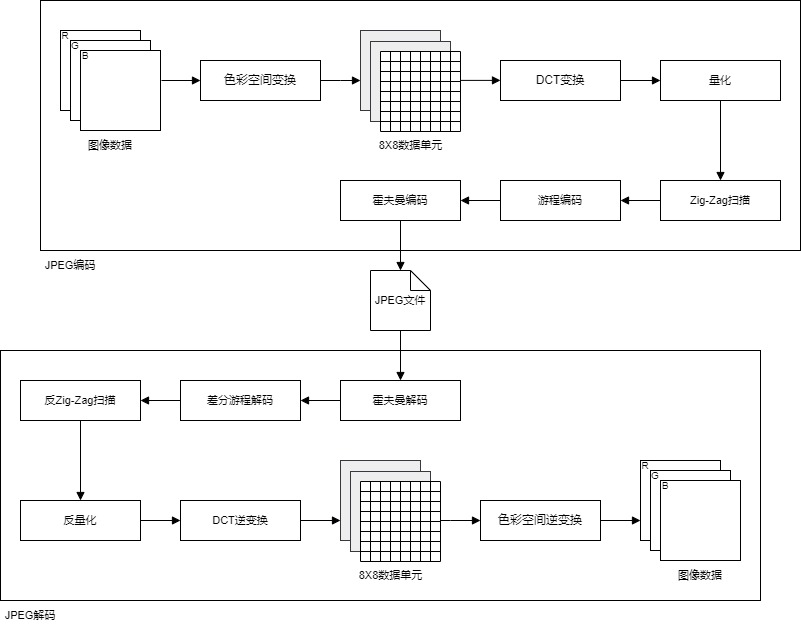
\includegraphics[scale=0.6]{./pictures/图片1.png}
    \caption{JPEG的编码和解码流程}\label{jpeg}
  \end{figure}
  JPEG格式的图像压缩流程为:首先将图像每个像素点的R、G、B颜色分量通过色彩空间变
  换转换成色度分量Cr、Cb以及亮度分量Y。之后将图片划分为若干个8*8的数据单元每个
  单元包含64个像素点,再对每个数据单元进行二维离散余弦变换(DCT),将二维的空间
  域数据变成二维的频域数据。再根据量化表对对应的频域分量进行量化处理。再通过Zig-Zag
  扫描将二维的频域数据转换成一维的序列。最后,依次通过游程编码和霍夫曼编码去除掉
  冗余的数据从而压缩JPEG图像数据。

  解压缩流程的流程与压缩的各个流程相反,除了量化和彩色空间变换这一过程会丢失一定
  的信息之外,其他的步骤都可以无损还原原数据,因此JPEG是一种有损压缩技术。

  下面依次对各个步骤做详细的描述。
  \subsection{彩色空间变换及逆变换}
    \vspace{1em}
    绝大多数的颜色都可以使用R、G、B三种颜色分量的线性组合进行合成。因此大多
    图像数据每个像素点都是以RGB分量表示。特别是再计算机视频技术中,不管使用
    哪种形式的彩色空间表示,最后一定要转换为RGB彩色空间显示。

    相关研究表明,人类的视觉系统有分别对红绿蓝三种颜色敏感层度的三种锥体细胞
    以及对明暗程度敏感的锥体细胞。其中对明暗程度的锥体细胞的数量大于对颜色敏
    感层度锥体细胞的数量。因此人类对是对色度辨识度大概是对明暗变换的辨识度的
    四分之一,因此可以利用对颜色感知强度的不同,将RGB彩色空间变换到YCrCb彩色
    空间再根据感知能力做对应的处理。

    ITU-R601建议规定的RGB彩色空间到YCbCr彩色空间变换关系如式(\ref{RGB2YCbCr}):
    \begin{equation}
      \begin{bmatrix}Y\\ Cr\\ Cb\end{bmatrix}=
      \begin{bmatrix}
        0.299 & 0.587 & 0.144\\
        0.500 & -0.419 & -0.081\\
        -0.169 & -0.331 & 0.500
      \end{bmatrix}
      \begin{bmatrix}R\\ G\\ B\end{bmatrix}+
      \begin{bmatrix}0\\ 128\\ 128\end{bmatrix}
      \label{RGB2YCbCr}
    \end{equation}

    在JPEG编码中,RGB颜色分量的取值范围通常是0到255,因此JPEG数据使用的是8位
    无符号整数。而在YCrCb颜色空间中,色度的颜色分量Cr、Cb的范围为-128到127。为
    了将其范围转换为0到255。故添加偏移量128,以确保范围在0到255内。这有助于在
    JPEG编码和解码中正确处理色度信息。这个偏移量是JPEG编码标准的一部分,确保
    了色度信息在JPEG图像中正确显示。

    彩色空间的逆变换如下式所示:
    \begin{equation}
      \begin{bmatrix}R\\ G\\ B\end{bmatrix}=
      \begin{bmatrix}
        1 & 1.402 & 0.\\
        1 & -0.344 & -0.714\\
        1 & 0 & 0.500
      \end{bmatrix}
      \begin{bmatrix}Y\\ Cb\\ Cr\end{bmatrix}+
      \begin{bmatrix}128\\ 128\\ 128\end{bmatrix}
      \label{YCbCr2RGB}
    \end{equation}

    由于人类的视觉系统对色度变化的感知低于亮度,因此在对色度分量进行采样的时
    候可以有选择性地进行降采样,进而降低数据量,这也是最朴素的图像压缩技术之
    一。根据对色度分量的采样率不同分为一下几种采样格式:
     
    YCbCr444:每个分量的采样率都为1。这意味着对于每一个像素点都进行完整的采
    样,携带完整的原图片信息,没有信息丢失。因此YCbCr44也是最高质量的采样格
    式。

    YCbCr422:在每两个水平相邻的像素中,只用一个Cr分量和一个Cb分量来表示该这
    两个像素点的色度分量,而每一个像素点都与之对应的Y分量。这种降采样的方式减
    少了颜色信息的存储和传输需求,在一定程度上牺牲了色度分辨率,但保留了较高
    的图像质量。

    YCbCr420:在每两个水平相邻以及垂直相邻的像素中,只用一个Cr分量和一个Cb分
    量表示这4个像素点的色度分量,而每一个像素点都有一个与之对应的Y分量。这种
    降采样的方式减少了存储和传输的需求,同时牺牲了色度的分辨率,是广泛应用与
    图片和视频压缩的以及传输的一种采样格式。本设计采用该采样格式。

    再经过采样后需要将采样得到的Y、Cb、Cr三种格式分别根据在空间上的分布整合成
    若干个8乘8的数据单元。该数据单元是之后JPEG编解码各个流程之中的处理单位,
    称为MCU(Minimun Coded Unit,最小编码单元)。当使用YCbCr422采样格式时单
    个MCU有2个8乘8的Y分量单元以及Cr和Cb分量8乘8单元各一个。同理,当使用YCbCr
    采样格式时单个MUC有4个8乘8的Y分量单元以及Cr和Cb分量8乘8单元各一个。
  \subsection{离散余弦变换及逆变换}
    \vspace{1em}
    由于人类的视觉系统在对,图像上亮度以及色度在空间上变化频率高的细节部分的注
    意力并不高,因此可以将图像上的高频率的信息适当的过滤掉,进而对数据进行近一
    步的压缩。DCT(Discrete Cosine Transform离散余弦变换)的作用是将图像从空间域
    转换到频域。在JPEG中,通过对每个MCU进行2D-DCT从而得到在空间上各个频率代
    表的正交基分量。2D-DCT的变换公式如下:
    \begin{equation}
      \begin{gathered}
        Y(u,v)=\alpha (u)\alpha (v) \sum_{i=0}^{N-1} \sum_{j=0}^{M-1}
        X(i,j)\cos \left[ \frac{\pi}{N}\left(i+\frac{1}{2}\right)u \right]
        \cos \left[ \frac{\pi}{M}\left(j+\frac{1}{2}\right)v \right]\\
        u=0,1,2,\cdots ,N-1 \\
        v=0,1,2,\cdots,M-1 \\
      \end{gathered}
      \label{2D-DCT}
    \end{equation}
    其中
    \begin{equation}
      \alpha (u) = \begin{cases}
        \sqrt{\frac{2}{N}} &,u>0\\
        \frac{1}{\sqrt{N}} &,u=0
      \end{cases}\quad
      \alpha (v) = \begin{cases}
        \sqrt{\frac{2}{M}} &,v>0\\
        \frac{1}{\sqrt{M}} &,v=0
      \end{cases}
    \end{equation}
    在JPEG中对8×8的像素块进行2D-DCT变换,所以有$N=8,M=8$ 。带入(\ref{2D-DCT})有:
    \begin{equation}
      \begin{gathered}
        Y(u,v)=\frac{1}{4}C(u)C(v) \sum_{i=0}^{7} \sum_{j=0}^{7}
        X(i,j)\cos \frac{(2i+1)u\pi}{16}\cos \frac{(2j+1)u\pi}{16}\\
        C (v),C (u) = \begin{cases}
          1 &,u,v>0\\
          \frac{1}{\sqrt{2}} &,u,v=0
        \end{cases}
      \end{gathered}
      \label{8*8 2D-DCT}
    \end{equation}
    在公式中,$f(i,j)$表示在位置$(i,j)$的像素值。其中$F(0,0)$实际上就是对64个像素点做
    加权平均,相当于8×8单元的平均亮度,成为DC(Direct coefficient,直流)系数。其余
    的63个频率值的点称为AC(Alternation coefficient,交流)系数。在交流系数中距离直流
    系数点越大代表该点的频率越高。

    将频域转换成空间域的变换称为IDCT(Inverse Discrete Cosine Transform,离散余弦逆变换)
    ,2D-IDCT的表达式如下:
    \begin{equation}
      \begin{gathered}
        X(i,j)=\frac{1}{4}\alpha(u)\alpha(v)\sum_{u=0}^{7}\sum_{v=0}^{7}
        Y(u,v)\cos\frac{(2i+1)u\pi}{16}\cos\frac{(2j+1)v\pi}{16}\\
          \alpha (v),\alpha (u) = \begin{cases}
            1 &,u,v>0\\
            \frac{1}{\sqrt{2}} &,u,v=0
          \end{cases}
      \end{gathered}
    \end{equation}
  \subsection{量化及反量化}
    \vspace{1em}
    量化是对DCT系数进行压缩的最关键一步,它按照给定的量化系数对每个DCT进行除法,
    再通过四舍五入取整数的方式得到量化后的系数,这个过程是一个一对多的映射过程。
    也就代表量化后的数据将无法完整地还原回来,因此存在数据丢失。这也是导致JPEG有
    损压缩的原因之一,量化的公式如下:
    \begin{equation}
      C(u,v)=round\left[\frac{F(u,v)}{Q(u,v)}\right]
    \end{equation}
    其中$F(u,v)$是2D-DCT系数,$Q(u,v)$是步长值,$C(u,v)$是量化后的值。而反量化
    自然就是将量化后的值乘回步长值,反量化的公式如下
    \begin{equation}
      F(u,v)=C(u,v)Q(u,v)
    \end{equation}

    量化是为了将大部分的高频分量都转换为0,进而减少高频分量的信息,同时也是为了
    下一步编码作出准备。通过不同的量化表从而控制图像的压缩程度。JPEG针对色度以及
    亮度有不同的量化表,如表\ref{亮度量化表}和表\ref{色度量化表}所示

    \begin{table}[H]
      \caption{亮度量化表}
      \label{亮度量化表}
      \centering
      \begin{tabular}{cccccccc}
        \toprule
        \multicolumn{8}{c}{亮度量化表}\\
        \midrule
        16 & 11 & 10 & 16 & 24 & 40 & 51 & 61 \\
        12 & 12 & 14 & 19 & 26 & 58 & 60 & 55 \\
        14 & 13 & 16 & 24 & 40 & 57 & 69 & 56 \\
        18 & 22 & 37 & 56 & 68 & 109 & 103 & 77 \\
        24 & 35 & 55 & 64 & 81 & 104 & 113 & 92 \\
        49 & 64 & 78 & 87 & 103 & 121 & 120 & 101 \\
        72 & 92 & 95 & 98 & 112 & 100 & 103 & 99 \\
        \bottomrule
      \end{tabular}
    \end{table}

    \begin{table}[H]
      \caption{色度量化表}
      \label{色度量化表}
      \centering
      \begin{tabular}{cccccccc}
        \toprule
        \multicolumn{8}{c}{色度量化表}\\
        \midrule
        17 & 18 & 24 & 47 & 99 & 99 & 99 & 99 \\
        18 & 21 & 26 & 66 & 99 & 99 & 99 & 99 \\
        24 & 26 & 56 & 99 & 99 & 99 & 99 & 99 \\
        47 & 66 & 99 & 99 & 99 & 99 & 99 & 99 \\
        99 & 99 & 99 & 99 & 99 & 99 & 99 & 99 \\
        99 & 99 & 99 & 99 & 99 & 99 & 99 & 99 \\
        99 & 99 & 99 & 99 & 99 & 99 & 99 & 99 \\
        99 & 99 & 99 & 99 & 99 & 99 & 99 & 99 \\
        \bottomrule
      \end{tabular}
    \end{table}

    对比两个表可以明显地看出,对于亮度步长的划分会更细一点,同时高频分量的
    值是普遍大于低频部分的。这是由于人眼对色度和高频部分图像信息的辨识能力
    低于亮度和高频部分。可以把量化当成一个在空间上的二维低通滤波器。
  \subsection{ZigZag扫描及反扫描}
    \vspace{1em}
    \begin{figure}[H]
      \centering
      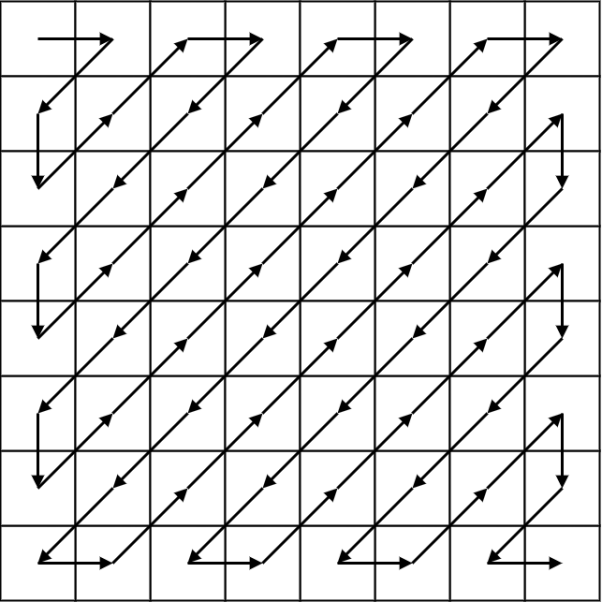
\includegraphics[scale=0.8]{./pictures/zigzag.png}
    \caption{ZigZag扫描}\label{zigzag}
    \end{figure}
    ZigZag扫描的过程如图\ref{zigzag}所示,它对8×8单元进行一维上的重排序。
    这一步骤也可以在量化前执行。对于大部分的8×8单元而言,在经过量化后,右
    下角的高频分量存在大量的零值。为了最大限度地将这些零值相邻为后面压缩做
    准备,通过Z字形扫描对8×8单元进行重排序。同理,反扫描即为将1维序列排回
    8×8单元。
  \subsection{熵编码及熵解码}
    \vspace{1em}
    图像数据的信息冗余量主要体现来两个层面:一是图像数据中各个相邻数据之间
    存在着一定的关联性。在一点体现在空间域上就是相邻的像素点之间的差距一般
    并不是很大,体现在频域上则是在经过量化和ZigZag扫描之后的数据中存在大量
    连续的零值;二是图像中不同的像素值的概率分布通常是不均匀的,某些像素值
    的出现的概率较高。如果对出现概率较高的数据采用跟少的位数进行编码,则能
    在一定程度减少一定的数据量。熵编码的主要目的为通过信息熵理论来减少这些
    冗余的信息,从而降低图像数据在传输和存储中所占用的时间和空间。同时熵编
    码是可逆的属于无失真压缩。

    在量化后。对于DC系数和AC系数两者在统计性质有很大的不同,因此采用两种不
    同的编码方式,对于DC系数采用差分脉冲编码(differential Pluse Code Modulaiton, DPCM)
    ,对于AC系数则使用游程编码(Run-Length Encodeing,RLE)。
    这两种编码方式通过在空间和频率上各个相邻数据的相似性的特点进行编码。在
    霍夫曼编码之前,能有效地减少图像数据的冗余性,以实现更高效的图像压缩。
    \subsubsection{DC系数差分脉冲编码}
    \vspace{1em}
      DC系数的值通常会比AC的值要大,而DC系数可以认为是每个8×8单元的平均值
      。而在空间上相邻的8×8单元平均值的差异通常不大。为了充分利用这一特点
      ,JPEG采用了差分脉冲编码,通过对当前的8×8单元的DC系数与前一个8×8单元
      的DC系数的差值进行编码。设$DC_{diff}$当前的8×8单元的DC系数$DC_{i}$减
      去前一个DC
      系数$DC_{i-1}$,$DC_{0}$表示第一个8×8单元的DC值。公式如下:
      \begin{equation}
        DC_{diff}=\begin{cases}
          DC_{i}-DC_{i-1} &,i>0\\
          DC_{0}&,i=0
        \end{cases}
      \end{equation}

      $DC_{diff}$的编码格式为(Size,Amplitude)。其中Size为Amplitude的位
      宽值,而Amplitude为$DC_{diff}$的幅值,当幅值为正是为原码。反正则为补
      码。因此Amplitude没有符号位。根据Size和Amplitude的第一位来判断
      $DC_{diff}$的正负。
    \subsubsection{AC系数游程编码}
      \vspace{1em}
      在经过ZigZag扫描之后,AC系数通常会出现大量连续的零值。也就可以通过连
      续0的个数来进行编码,这种方式称为游程编码。游程编码可以有效地表示续
      出现的相同的值,用该数值本事加上该数值的重复次数来替代。进而减少数据
      量来做到数据压缩。游程编码的编码格式为(Run,Size,Amplifier)。其中
      Run(游程)表示非零值前面零值的个数,Size表示非零值的尺寸,Amplifier      表示非零值的幅值。同理,也可以根据这三个值还原回原码,从而做到解码。

      有两种特殊的情况需要注意:当出现从某个非零值直到最后第64个值都为零时
      的情况,使用0/0(EOB)
      进行编码。当连续零值的数量超过16个时,使用F0(ZRL)进行编码。
    \subsubsection{霍夫曼编码}
      \vspace{1em}
      霍夫曼编码是一种可变长度编码,这种编码方法由霍夫曼(Huffman)在1952
      年提出。它根据字符的出现的概率来构建编码映射。以实现码字的平均长度最
      短。该编码方式的压缩率接近香农所定义的极限压缩率,因此这种方法也称为
      最佳编码。
      通过查找AC和DC系数对应颜色分量的Huffman表进行编码。Huffman码表是由JP
      EG标准通过大量的图像数据统计进而规定的,详细内容如下表所示。
      \begin{table}[H]
        \centering
        \caption{亮度$DC_{diff}$Huffman表}
        \begin{tabular}{ccc}
          \toprule
          尺寸  & Huffman码长度 & Huffman码字\\
          \midrule
          0     & 2             & 00\\
          1     & 3             & 010\\
          2     & 3             & 011\\
          3     & 3             & 100\\
          4     & 3             & 101\\
          5     & 3             & 110\\
          6     & 4             & 1110\\
          7     & 5             & 11110\\
          8     & 6             & 111110\\
          9     & 7             & 1111110\\
          A     & 8             & 11111110\\
          B     & 9             & 111111110\\
          \bottomrule
        \end{tabular}
      \end{table}

      \begin{table}[H]
        \centering
        \caption{色度$DC_{diff}$Huffman表}
        \begin{tabular}{ccc}
          \toprule
          尺寸  & Huffman码长度 & Huffman码字\\
          \midrule
          0     & 2             & 00\\
          1     & 3             & 010\\
          2     & 3             & 011\\
          3     & 3             & 100\\
          4     & 3             & 101\\
          5     & 3             & 110\\
          6     & 4             & 1110\\
          7     & 5             & 11110\\
          8     & 6             & 111110\\
          9     & 7             & 1111110\\
          A     & 8             & 11111110\\
          B     & 9             & 111111110\\
          \bottomrule
        \end{tabular}
      \end{table}

      \begin{table}[H]
        \centering
        \caption{亮度AC系数Huffman表}
        \begin{tabular}{ccc}
          \toprule
          游程/尺寸 & Huffman码长度 & Huffman码字\\
          \midrule
          0/0(EOB)  & 4             & 1010\\
          0/1       & 2             & 00\\
          0/2       & 2             & 01\\
          0/3       & 3             & 100\\
          0/4       & 4             & 1011\\
          0/5       & 5             & 11010\\
          0/6       & 7             & 1111000\\
          0/7       & 8             & 11111000\\
          0/8       & 10            & 1111110110\\
          0/9       & 16            & 1111111110000010\\
          0/A       & 16            & 1111111110000011\\
          1/1       & 4             & 1100\\
          $\cdots$  & $\cdots$      & $\cdots$\\
          F/A       & 16            & 1111111111111110\\
          \bottomrule
        \end{tabular}
      \end{table}

      \begin{table}[H]
        \centering
        \caption{色度AC系数Huffman表}
        \begin{tabular}{ccc}
          \toprule
          游程/尺寸 & Huffman码长度 & Huffman码字\\
          \midrule
          0/0(EOB)  & 2             & 00\\
          0/1       & 2             & 01\\
          0/2       & 3             & 100\\
          0/3       & 4             & 1010\\
          0/4       & 5             & 11000\\
          0/5       & 5             & 11001\\
          0/6       & 6             & 111000\\
          0/7       & 7             & 1111000\\
          0/8       & 9             & 111110100\\
          0/9       & 10            & 1111110110\\
          0/A       & 12            & 111111110100\\
          1/1       & 4             & 1011\\
          $\cdots$  & $\cdots$      & $\cdots$\\
          F/A       & 16            & 1111111111111110\\
          \bottomrule
        \end{tabular}
      \end{table}

      在解码时,当多个Huffman串行码流排列输出在一起时,可以使用二叉树解索
      引从而获取对应原码从而做到解码得到尺寸,再通过尺寸得到幅值所占的的位
      宽得到幅值。通过这种方式从而区分出码流中的各个像素点的数据。
      \begin{figure}[H]
        \centering
        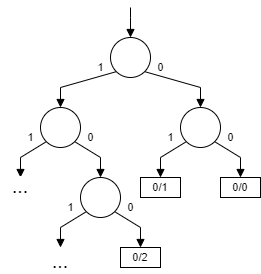
\includegraphics[scale=0.8]{./pictures/deCodeTree.png}
        \caption{通过二叉树解码}
      \end{figure}
  \subsection{JPEG文件格式}
    \vspace{1em}
    通过上述过程得到了压缩之后的图像数据,除此之外,要对数据进行解码。还需
    要知道图像的相关属性等信息。JPEG委员会在指定JPEG标准时,定义了许多用来
    区分图像数据及其相关信息的文件格式。目前,使用比较广泛的是1992年9月由E
    ric Hamilton 提出的JPEG文件交换格式JFIF(JPEG File Interchange Format)
    1.02版本。大多数的设备都支持JFIF文件交换格式。JPEG编码的最后一个步骤就是把各
    种标记代码和编码后的图像数据组成一帧一帧的位码流,这样就方便传输、存储
    和解码器译码。

    JFIF文件格式可以分为两个部分:标识和压缩数据。每个标识的前一个字节是固
    定值0xFF。每个标记之前还可以添加数量不限的0xFF。下表列举几种常见的标记
    码以及它们各自的数据结构。
    \begin{table}[H]
      \centering
      \caption{几种常见的标记}
      \begin{tabular}{cc}
        \toprule
        标记种类 & 含义\\
        \midrule
        SOI & 图像的开始\\
        APP0 & JFIF引用的数据块\\
        SOF0 & 帧开始\\
        DHT & Huffman表\\
        SOS & 扫描线开始\\
        EOI & 图像结束\\
        \bottomrule
      \end{tabular}
    \end{table}
    
    \begin{table}[H]
      \centering
      \caption{APP0标识}
      \begin{tabular}{ccc}
        \toprule
        标识结构 & 字节数 & 含义\\
        \midrule
        0xFF & 1 & \multirow{2}{*}{APP0标识}\\
        0xE0 & 1 &\\
        \bottomrule
      \end{tabular}
    \end{table}

    \begin{table}[H]
      \centering
      \caption{OF0标识}
      \begin{tabular}{ccc}
        \toprule
        标识结构 & 字节数 & 含义\\
        \midrule
        0xFF & 1 & \multirow{2}{*}{APP0标识}\\
        0xC0 & 1 &\\
        $L_{f}$ & 2 & 长度字段,表示图像帧信息长度\\
        P & 1 & 指每个像素点的颜色信息的宽度,通常是8位或12位\\
        Y & 2 & 图像的高度\\
        X & 2 & 图像的宽度\\
        $N_{f}$ & 1 & 图像颜色通道的数量。通常为1或3,分别表示灰度图和RGB彩色图\\
        $N_{NT}$ & 1 & 颜色通道,0表示Y通道,1表示Cb通道,2表示Cr通道\\
        $H_{TN}Y_{TN}$ & 1 & 水平方向和垂直方向的采样率\\
        $T_{QNT}$ & 1 & 表示使用的Huffman编码表的编号\\
        \bottomrule
      \end{tabular}
    \end{table}

    \begin{table}[H]
      \centering
      \caption{DHT标识}
      \begin{tabular}{ccc}
        \toprule
        标识结构 & 字节数 & 含义\\
        \midrule
        0xFF & 1 & \multirow{2}{*}{APP0标识}\\
        0xC4 & 1 &\\
        $L_{b}$ & 2 & 长度字段,表示Huffman码字段的长度\\
        $T_{c}$ & 0.5 & 当为1时,表示使用该表处理AC系数,为0时,表示该表处理DC系数\\
        $T_{b}$ & 0.5 & 表示Huffman表的编号\\
        $L_{i}$ & 1 & Huffman表的长度统计,用于表示不同码字长度的符号数目,i从1到16\\
        $V_{ij}$ & 1 & 代表每一个Huffman码表所代表的值\\
        \bottomrule
      \end{tabular}
    \end{table}

    \begin{table}[H]
      \centering
      \caption{SOS标识}
      \begin{tabular}{ccc}
        \toprule
        标识结构 & 字节数 & 含义\\
        \midrule
        0xFF & 1 & \multirow{2}{*}{APP0标识}\\
        0xDA & 1 &\\
        $L_{s}$ & 2 & 长度字段,表示数据内容的长度\\
        $N_{s}$ & 1 & 表示扫描所涉及到颜色通道的数量\\
        $C_{s}N_{s}$ & 0.5 & 表示Scan中成分的编号\\
        $T_{d}N_{s}$,$T_{a}N_{s}$ & 1 & $T_{a}N_{s}$表示数据的高4位$T_{a}N_{s}$表示数据的低4位\\
        $S_{s}$ & 1 & 一般为0\\
        $S_{s}$ & 1 & 一般为63\\
        $A_{b}$,$A_{l}$ & 1 & 一般为0\\
        \bottomrule
      \end{tabular}
    \end{table}

    \begin{table}[H]
      \centering
      \caption{EOI标识}
      \begin{tabular}{ccc}
        \toprule
        标识结构 & 字节数 & 含义\\
        \midrule
        0xFF & 1 & \multirow{2}{*}{EOI标识}\\
        0xD9 & 1 &\\
        \bottomrule
      \end{tabular}
    \end{table}
  \subsection{本章总结}
    \vspace{1em}
    本章阐述了JPEG图像数据编解码的原理和相关理论,以及各个执行的步骤。

\newpage
\section{JPEG编码系统硬件结构设计}
  \vspace{1em}
  上一章节讲解了JPEG编码的步骤和过程。这一章讲解本设计如何使用硬件实现JPEG
  的编码以及解码。内容包含数字电路设计中的一些设计思想,编码系统的结构划分
  ,以及各个模块的结构和运行原理。
  \subsection{设计思想}
    \vspace{1em}
    在数字系统设计中,一个经常围绕的问题就是速度和面积的权衡。使用多个处理
    单元对数据进行处理是一种朴素的提高系统计算速度和吞吐量的方式。与之带来
    的副作用就是电路面积的增大。面积增大所带来的副作用不仅仅是成本增加的问
    题,它也伴随着系统功耗和发热量的增加,这些负面影响都会降低系统的稳定性
    。而有些运算过程数据依赖性高、并行操作无法有效地提高性能。甚至可能因为
    额外的开销导致性能的下降。因此,一个好的数字系统设计往往能够权衡速度和
    面积。

    通过前人的大量经验实践总结出了大量的设计思想。如果能在合适的情况下使用
    这些设计思想,就能得到一个好的设计。下面描述变设计所使用的几种设计思想
    。
    \subsubsection{流水线}
      \vspace{1em}
      如果一个运行周期长的操作的运行过程能个分解成一各个子步骤。并将这些子
      步骤封装成一个个并行的模块。让每个操作的不同步骤在不同时刻错开运行,
      每个模块同时执行不同操作所对应的步骤。最终每经过一个子步骤的时间,就
      可以得到一个操作的运行结果,通过这种方式系统的吞吐量能得到大幅度提高
      ,在运行过程中每个步骤的结果数据一步步的从输入流动到输出,因此该操作
      得名流水线(Pilpeline)。这种方式在如今的工厂车间运用广泛。

      下面通过对比一个分3个步骤的执行的例子,来分析流水线所带来的性能的提
      升。假设一个系统的执行需要通过步骤一、步骤二、步骤三三个步骤的到结果,
      每个步骤所花费的时间为一个时钟周期。如果依次按照顺序完成N次运算,每
      隔3个时钟周期得到一个运行结果,完成所有运算所花费的时间就是3N。如果
      设置三个执行不同步骤的模块同时并行执行,且每个模块执行不同操作的步骤
      ,如第一个时刻执行步骤一的模块执行操作一的步骤一,如第二个时刻执行步
      骤一的模块执行操作二的步骤一,执行步骤二的模块执行操作一的步骤二;第
      三个时刻执行步骤一的模块执行操作三的步骤一,执行步骤二的模块执行操作
      二的步骤二,执行步骤三的模块执行操作一的步骤三;之后N个时刻以此类推
      在第4个时刻得到操作一的结果,下一时刻得到操作二的结果。之后每经过一
      个时刻得到一个操作结果。得到N操作的结构则需要花费3+N个时钟周期的时间
      。通过这种方式显著地提升数据的吞吐量。
      \begin{figure}[H]
        \centering
        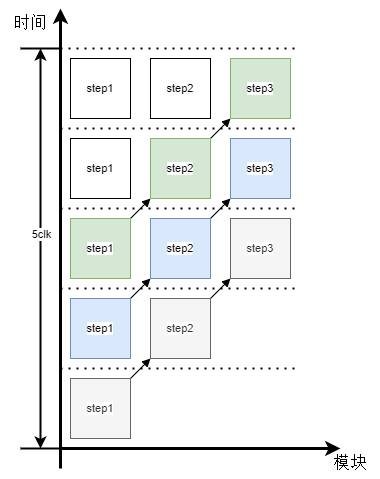
\includegraphics[scale=0.6]{./pictures/流水线.png}
        \caption{流水线操作}
      \end{figure}

      除此之外,流水线通常用于提高数字电路的最大运行时钟频率。在时序电路中
      时钟周期至少要大于保持时间、建立时间、组合逻辑延迟时间三者之和。而组
      合逻辑延迟时间取决于组合逻辑中最长的电路路径。如果在组合逻辑之中插入
      寄存器,从而切分组合逻辑的关键路径,使组合逻辑在每个时钟周期安装流水
      线的方式运行。通过这种方式提高时序电路的最大运行时钟频率。从而提高整
      个电路的运算速度。
      \subsubsection{脉动阵列}
        \vspace{1em}
        脉动阵列(Systolic Array)是一种由众多简单的运算元件(Processing 
        Element,PE)按照一定的规则排列的硬件架构。它最早由H.T.
        Kung在1982年提出。一个脉动阵列具备一下特征:

        (1)由单一或多种构造的PE按照规则排列;

        (2)只有相邻的PE互相连接,数据只能通过在局部范围内移动;

        (3)PE只重复进行简单的数据处理和必要的数据收发;

        (4)所有PE由统一的时钟同步工作;

        每个PE都和相领的PE同步进行数据收发和运算。数据从外部流入,PE阵列一
        边搬运数据,一边采用流水线或并行的方式对其进行处理。各个PE的运算和
        数据的收发动作和心脏规律地收缩促使血液流动的过程非常相似,因此得称
        脉动阵列。

        由于脉动阵列的数据移动只在相邻的PE中进行,这种方式有利于芯片或FPGA
        的布局步线,脉动阵列根据排列和连接方式,主要可分为串行的一维脉动阵
        列,网格连接的二维脉动阵列。其中一维的脉动阵列能实现FIR滤波器,向
        量乘法,数据排序。二维脉动阵列能完成矩阵运算,如图\ref{2D array}。
        \begin{figure}[H]
          \centering
          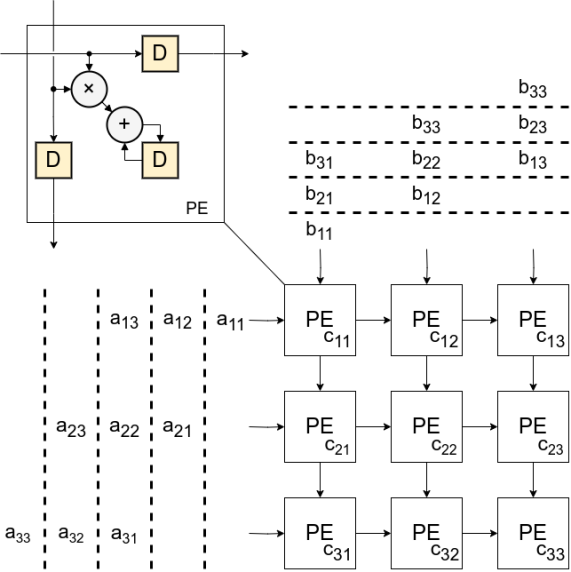
\includegraphics[scale=1]{./pictures/2Darray.png}
          \caption{二维脉动技术矩阵乘法}
          \label{2D array}
        \end{figure}

        \subsubsection{乒乓操作}
          \vspace{1em}
          在两个功能模块进行数据传输时,如果两个模块的吞吐量不同,对数据接
          收的顺序存在差异等原因。导致两个模块不能够同时工作。这个情况下就
          可以在两个模块之间添加乒乓缓存(Ping-pong 
          buffer)来解决这个问题,这种解决方法被称为乒乓操作。

          乒乓操作的处理流程,在两个模块之间添加2个buffer,来进行缓存数据
          。这个buffer通常是FIFO(First in first 
          out,先入先出队列)或者RAM。初始状态下,数据发送模块先向一个buff
          er写入发送的数据,当buffer的容量满后,数据接收模块开始向这个buff
          er读出数据。同时数据模块继续向另外一个buffer进行写入。之后依次类
          推,两个buffer交错读写。这样,只有在初始时数据发送模块在往第一个
          buffer写入数据时,接收模块是空闲状态,在其余时间内,两个模块都是
          同时工作的。
          \begin{figure}[H]
            \centering
            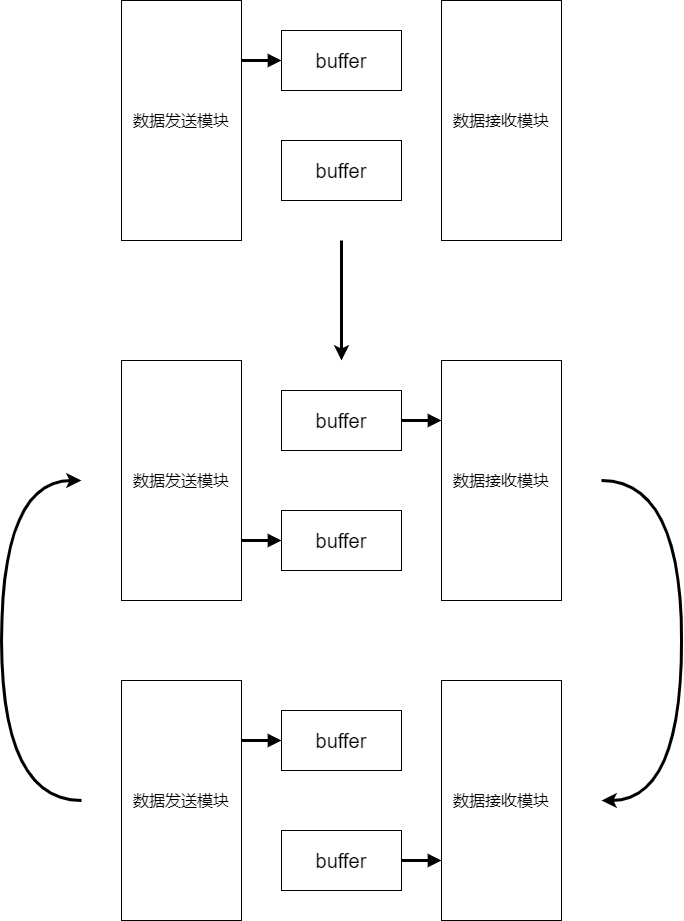
\includegraphics[scale=0.3]{./pictures/乒乓操作.png}
            \caption{乒乓操作}
            \label{2D array}
          \end{figure}
  \subsection{编码模块划分}
    \vspace{1em}
    \begin{figure}[H]
      \centering
      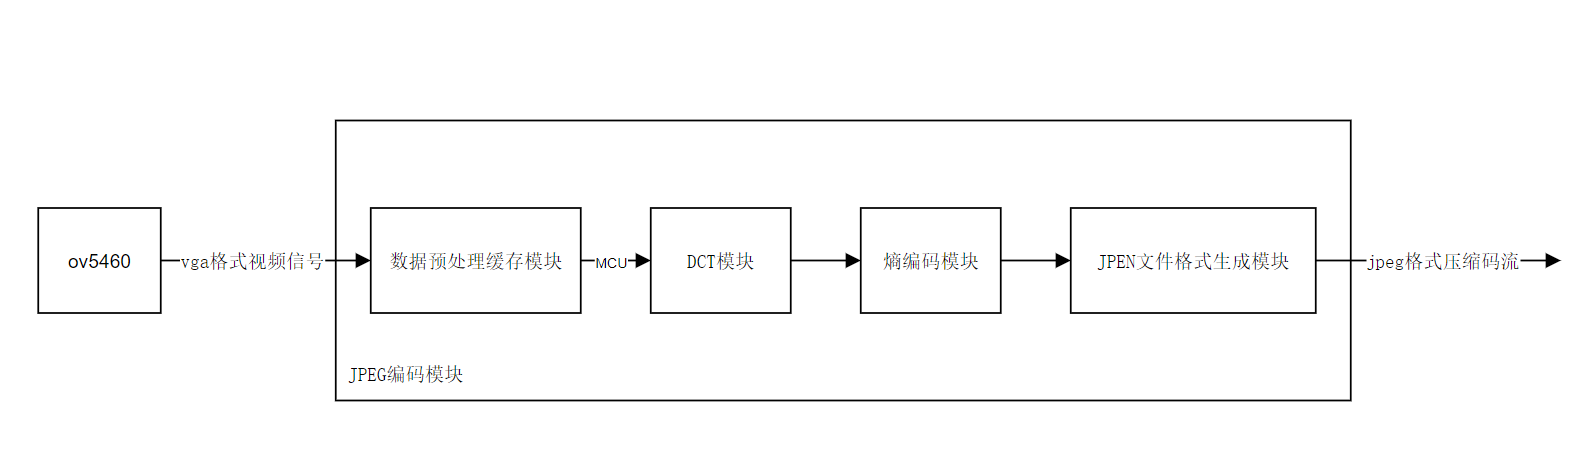
\includegraphics[scale=0.3]{./pictures/编码模块.png}
      \caption{编码模块}
      \label{code module}
    \end{figure}
    JPEG编码模块的内部模块划分如图\ref{code 
    module},它接收ov5460CMOS图像传感器的vga格式的视频信号。输出jpeg格式的
    压缩码流。视频信号依次经过数据预处理缓存模块、DCT模块、熵编码模块、JPE
    G文件格式生成模块。下面的小节详细介绍这4个模块。
  \subsection{DCT模块}
    \vspace{1em}
    DCT模块接收数据预处理模块输出的,Y、Cr、Cb三个颜色通道的8*
    8像素单元。并对每个颜色通道实现进行DCT、量化、Zigzag扫描这三个步骤。
    \begin{figure}[H]
      \centering
      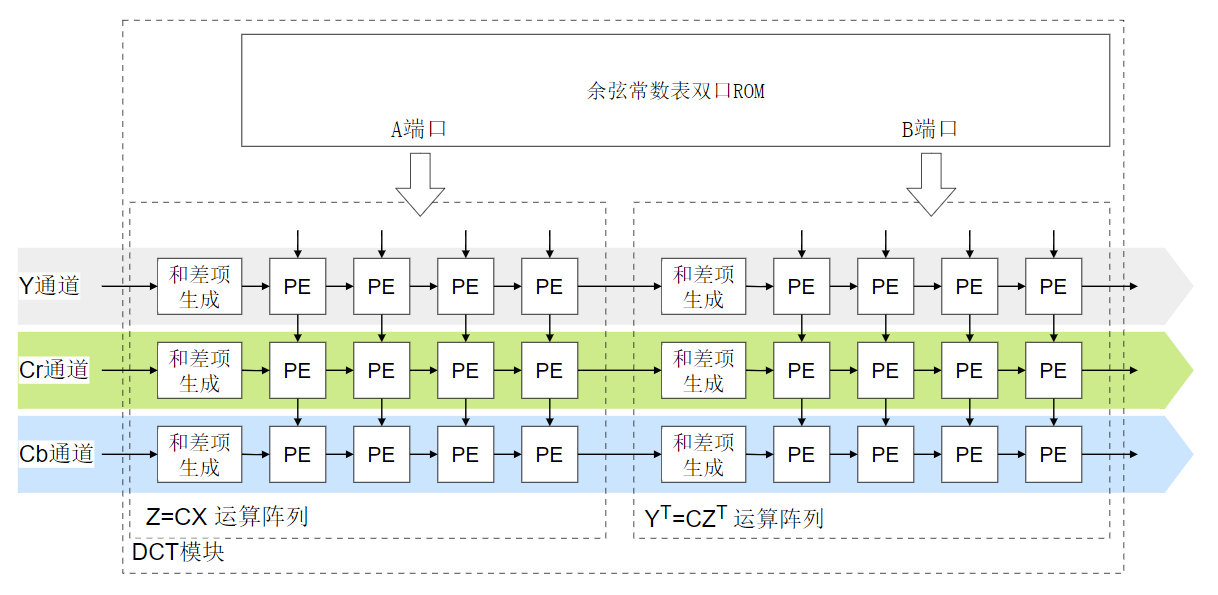
\includegraphics[scale=0.5]{./pictures/dct.png}
      \caption{DCT模块内部结果}
      \label{code module}
    \end{figure}

    由于本设计采用的采样格式为YCrCb420,所以在每个MCU中有一个Cr分量8×8像素
    单元,一个Cb分量8×8像素单元,和4个Y分量8×8像素单元。因此Cr和Cb可以分时
    复用同个色度通道,每个通道的DCT和量化模块均相同。

    如果根据2D-
    DCT原公式(\ref{8*8 2D-DCT}),对单个8×8单元进行运算,需要进行4096次乘法和4096次加法加法运算。需要
    使用较多的大量的乘法器资源,而乘法器资源在fpga中比较稀缺。为了降低计算
    的复杂度,本设计使用了DA算法,通过行列分解2D-DCT运算。
    \subsection{DA算法}
      \vspace{1em}
      根据式(\ref{8*8 2D-DCT})的特征可以根据行和列分解成两次一维的DCT变换,
      计算过程如下:
      \begin{equation*}
        \begin{aligned}
          Y(u,v)&=\frac{1}{4}C(u)C(v)\sum_{i=0}^{7}\sum_{j=0}^{7}X(i,j)
          \cos\frac{(2i+1)u\pi}{16}\cos\frac{(2j+1)v\pi}{16}\\
          Y(u,v)&=\frac{1}{2}C(u)\sum_{i=0}^{7}\cos\frac{(2i+1)u\pi}{16}
          \frac{1}{2}C(v)\sum_{j=0}^{7}X(i,j)\cos\frac{(2j+1)v\pi}{16}
        \end{aligned}
      \end{equation*}
      令
      \begin{equation}
        Z(i,v)=\frac{1}{2}C(v)\sum_{j=0}^{7}X(i,j)\cos\frac{(2j+1)v\pi}{16}
        \label{colDCT}
      \end{equation}
      有
      \begin{equation} 
        Y(u,v)=\frac{1}{2}C(u)\sum_{i=0}^{7}
        Z(i,v)\cos\frac{(2i+1)u\pi}{16}
        \label{rowDCT}
      \end{equation}

      下面再将式(\ref{colDCT})和式(\ref{rowDCT})整理成矩阵运算,令$C$为带
      常数项的系数矩阵,则有
      \begin{equation}
        C=\begin{bmatrix}
          a & a   & a   & a   & a   & a   & a   & a\\
          b & d   & e   & g   & -g  & -e  & -d  & -b\\
          c & f   & -f  & -c  & -c  & -f  & f   & c\\
          d & -g  & -b  & -e  & e   & b   & g   & -d\\
          a & -a  & -a  & a   & a   & -a  & -a  & a\\
          e & -b  & g   & d   & -d  & -g  & b   & -e\\
          f & -c  & c   & -f  & -f  & c   & -c  & f\\
          g & -e  & d   & -b  & b   & -d  & e   & -g\\
        \end{bmatrix},
        \begin{bmatrix}
          a \\ b \\ c \\ d \\ e \\ f \\ g
        \end{bmatrix}=
        \frac{1}{2}\begin{bmatrix}
          \cos(4\pi/16)\\
          \cos(\pi/16)\\
          \cos(2\pi/16)\\
          \cos(3\pi/16)\\
          \cos(4\pi/16)\\
          \cos(5\pi/16)\\
          \cos(6\pi/16)\\
          \cos(7\pi/16)\\
        \end{bmatrix}
        \label{C}
      \end{equation}
      则式(\ref{colDCT})和式(\ref{rowDCT})的矩阵形式分别为
      \begin{equation}
        Z=CX 
        \label{col}
      \end{equation}
      \begin{equation}
        Y=(CZ^{T})^{T}
      \end{equation}
      整理得
      \begin{equation}
        Y^{T}=C(CX)^{T} 
        \label{rowColDCT}
      \end{equation}
      通过上述步骤,将8×8的2D-DCT分解成两次对$C$的左乘运算。对于Z的每个列
      向量有
      \begin{equation}
        \begin{bmatrix}
          z_{i0}\\z_{i1}\\z_{i22}\\z_{i3}\\z_{i4}\\z_{i5}\\z_{i6}\\z_{i7}
        \end{bmatrix}=\begin{bmatrix}
          a & a   & a   & a   & a   & a   & a   & a\\
          b & d   & e   & g   & -g  & -e  & -d  & -b\\
          c & f   & -f  & -c  & -c  & -f  & f   & c\\
          d & -g  & -b  & -e  & e   & b   & g   & -d\\
          a & -a  & -a  & a   & a   & -a  & -a  & a\\
          e & -b  & g   & d   & -d  & -g  & b   & -e\\
          f & -c  & c   & -f  & -f  & c   & -c  & f\\
          g & -e  & d   & -b  & b   & -d  & e   & -g\\
        \end{bmatrix}\begin{bmatrix}
          x_{i0}\\x_{i1}\\x_{i22}\\x_{i3}\\x_{i4}\\x_{i5}\\x_{i6}\\x_{i7}
        \end{bmatrix}
        \label{colDCTCol}
      \end{equation}
      观察到$C$具有左右对称的性质,可将(\ref{colDCTCol})分解如下
      \begin{equation}
        \begin{bmatrix}
          z_{i0}\\z_{i2}\\z_{i4}\\z_{i6}\\
        \end{bmatrix}=\begin{bmatrix}
          a & a   & a   & a\\
          c & f   & -f  & -c\\
          a & -a  & -a  & a\\
          f & -c  & c   & -f\\
        \end{bmatrix}\begin{bmatrix}
          x_{i0}+x_{i7}\\
          x_{i1}+x_{i6}\\
          x_{i2}+x_{i5}\\
          x_{i3}+x_{i4}\\
        \end{bmatrix}, 
        \begin{bmatrix}
          z_{i1}\\z_{i3}\\z_{i5}\\z_{i7}\\
        \end{bmatrix}=\begin{bmatrix}
          b & d   & e   & g\\
          d & -g  & -b  & -e\\
          e & -b  & g   & d\\
          g & -e  & d   & -b\\
        \end{bmatrix}\begin{bmatrix}
          x_{i0}-x_{i7}\\
          x_{i1}-x_{i6}\\
          x_{i2}-x_{i5}\\
          x_{i3}-x_{i4}\\
        \end{bmatrix}
      \end{equation}
      $Z$每个列向量的偶项等于$x_{n}+x_{7-n}$(下面统称为和项)的线性组合,
      奇项等于$x_{n}-x_{7-n}$的线性组合。对于$Y_{T}=CY_{T}$也是同理。

      通过上述步骤将8乘8的矩阵运算转换为两次4乘4的矩阵运算。减少了计算的复
      杂度减少了一倍。为了在硬件中使用定点数运算,将中各个系数都扩大210倍
      并取整。

    \subsection{DA算法的硬件实现}
      \vspace{1em}
      对于DA算法中2次4乘以4的矩阵运算,提出了一种基于脉动阵列的硬件实现。
      如图\ref{DCT脉动阵列}所示,使用二维脉动阵列实现DA算法中的$Z=CX$计算。
      \begin{figure}[H]
        \centering
        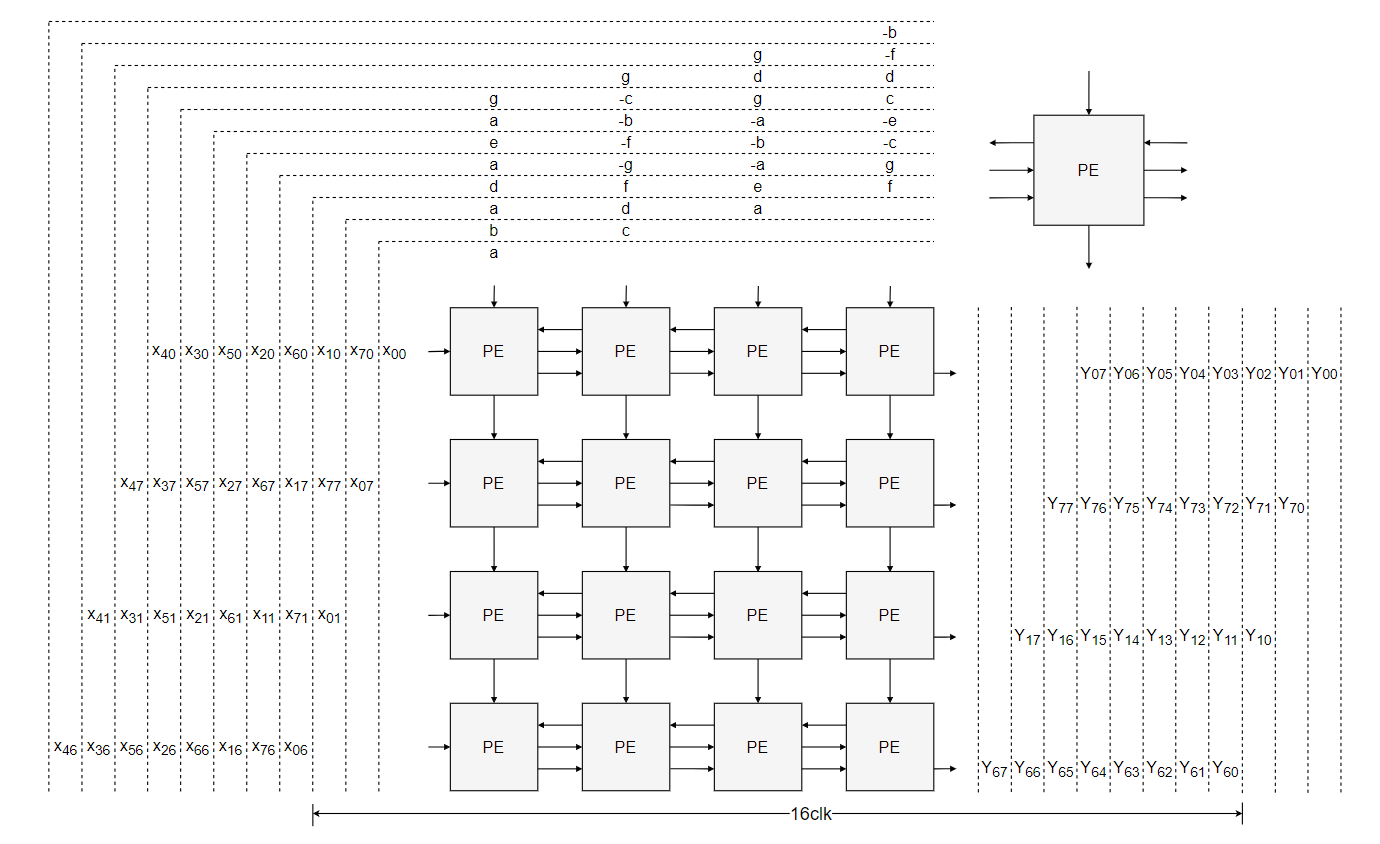
\includegraphics[scale=0.4]{./pictures/DCT脉动阵列.png}
        \caption{计算$Z=CX$的二维脉动阵列实现}
        \label{DCT脉动阵列}
      \end{figure}
      该脉动阵列的PE内部结果如图\ref{PE}所示
      \begin{figure}[H]
        \centering
        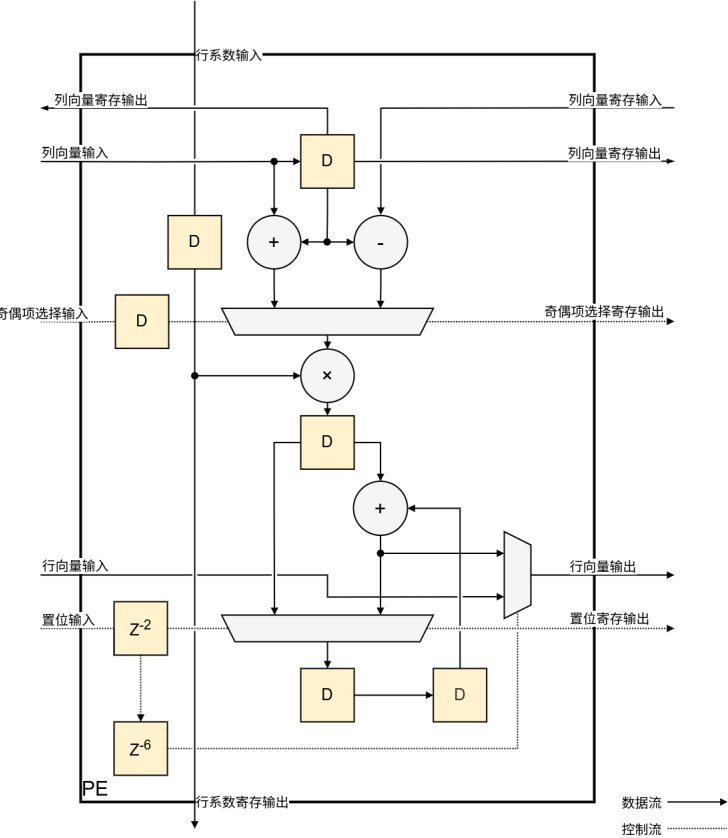
\includegraphics[scale=0.3]{./pictures/DCT_PE.png}
        \caption{PE的内部结构}
        \label{PE}
      \end{figure}
      \begin{figure}[H]
        \centering
        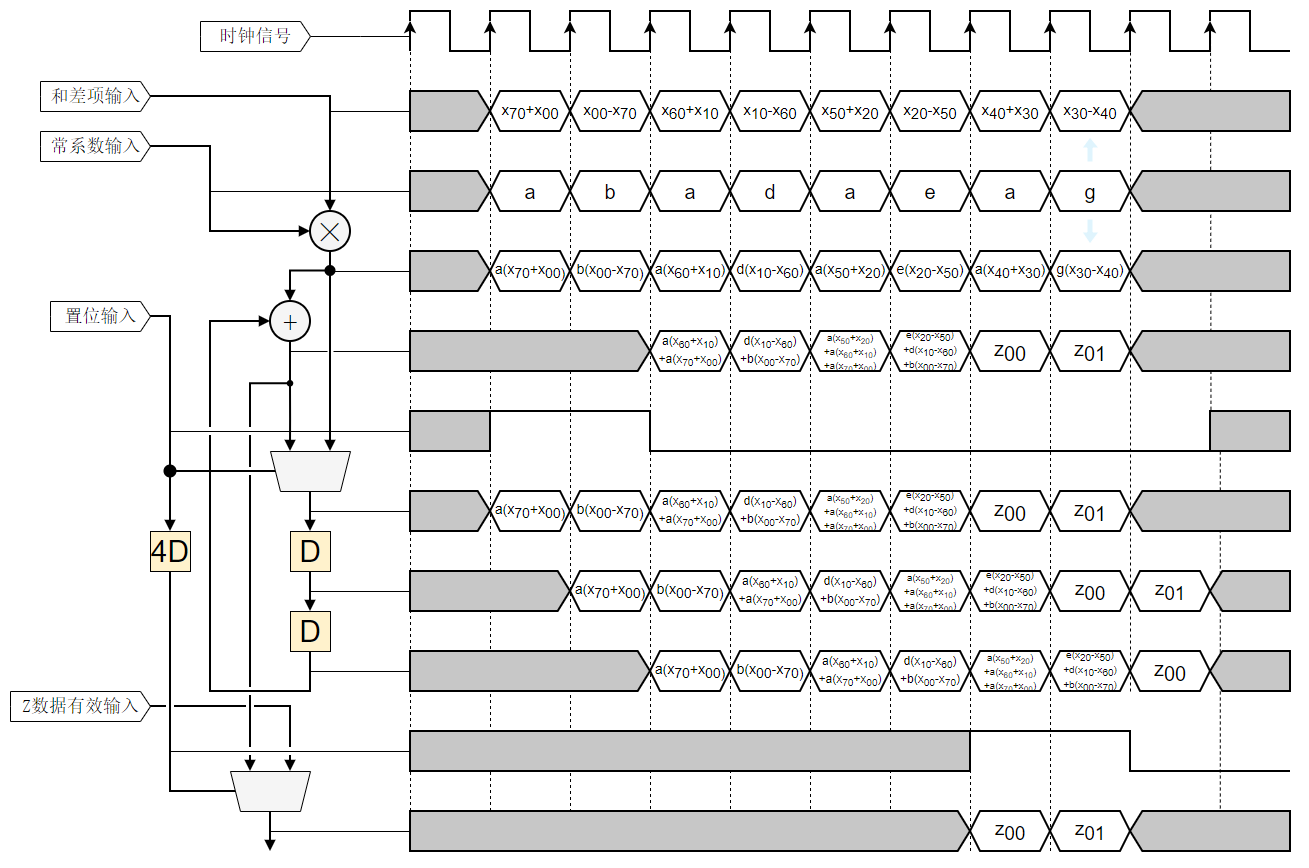
\includegraphics[scale=0.35]{./pictures/PE时序.png}
        \caption{PE运行时序}
        \label{PE运行时序}
      \end{figure}
      以列向量输入$x_{00},x_{01},x_{02},x_{03},x_{04},x_{05},x_{06},x_{07}$
      计算输出$z_{01},z_{02}$的
      过程为例,描述单个PE的运行原理。首先将列向量通过依次通过2个寄存器延
      迟2个时钟周期,使相邻的列向量分量能够同时并行输出。为了减少资源浪费
      ,其中第二个寄存器来自水平相邻的PE。通过当前输入与延迟1拍输入送至加
      法器得到和项。延迟1拍和延迟2拍送至加法器得到差项。其中正确的和项差
      项在每个时钟周期中错开。为了使yij的偶项和奇项的计算能够复用同一个乘
      法器,将加法器和减法器的输出送入到一个2选1多路选择器,再将其输入对
      应行系数相乘的得到每一个乘项。得到乘项后将其送入寄存器,当乘项是输
      出项的第一个乘项时,直接输入该乘项。否则和之前的乘项一起输入到加法
      进行累加。该过程通过置位信号控制2选1多路选择器实现。使用2个串联的寄
      存器使奇项和偶项的运算时序能够对齐。当累加到4个乘项时,即计算出
      $z_{01},z_{02}$
      。从$x_{00}$到$z_{00}$一个需要8个时钟周期。将置位信号延迟8拍作为最
      后输出2选1多路选择器的选择输入。具体的运行时序如图\ref{PE运行时序}
      所示。

      由于本设计编码模块输入的是像素点串行的vga格式信号。如果使用4×4二维
      脉动阵列进行运算,则该模块的吞吐量是输入数据吞吐量的4倍。这代表该模
      块在每个运行周期会有四分之三运行周期的空闲时间,模块的处理数据的速
      率已经饱和。为了不浪费资源,如图\ref{一维脉动阵列}所示只使用4个PE组
      成一行的一维脉动阵列进行运算。这样面积和速度的取舍能做到最优。
      \begin{figure}[H]
        \centering
        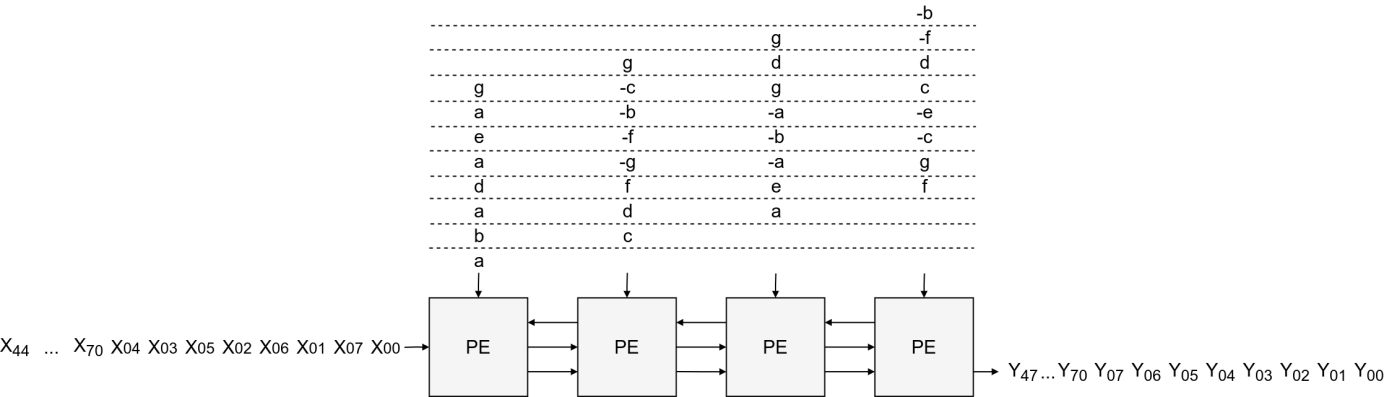
\includegraphics[scale=0.8]{./pictures/1D-DCT.png}
        \caption{一维脉动阵列}
        \label{一维脉动阵列}
      \end{figure}

      通过上述过程可以得到$Z$,还需要再计算$Y^{T}=CZ^{T}$,上述模块依次输出
      $Z$的列向量$Z_{0},Z_{7},Z_{1},Z_{6},Z_{2},Z_{5},Z_{3},Z_{4}$
      所以需要通过$Z_{n},Z_{7-n}$得到$Z^{T}$
      的差项和和项。使用如图\ref{和差项生成}所示的电路结构得到。
      \begin{figure}[H]
        \centering
        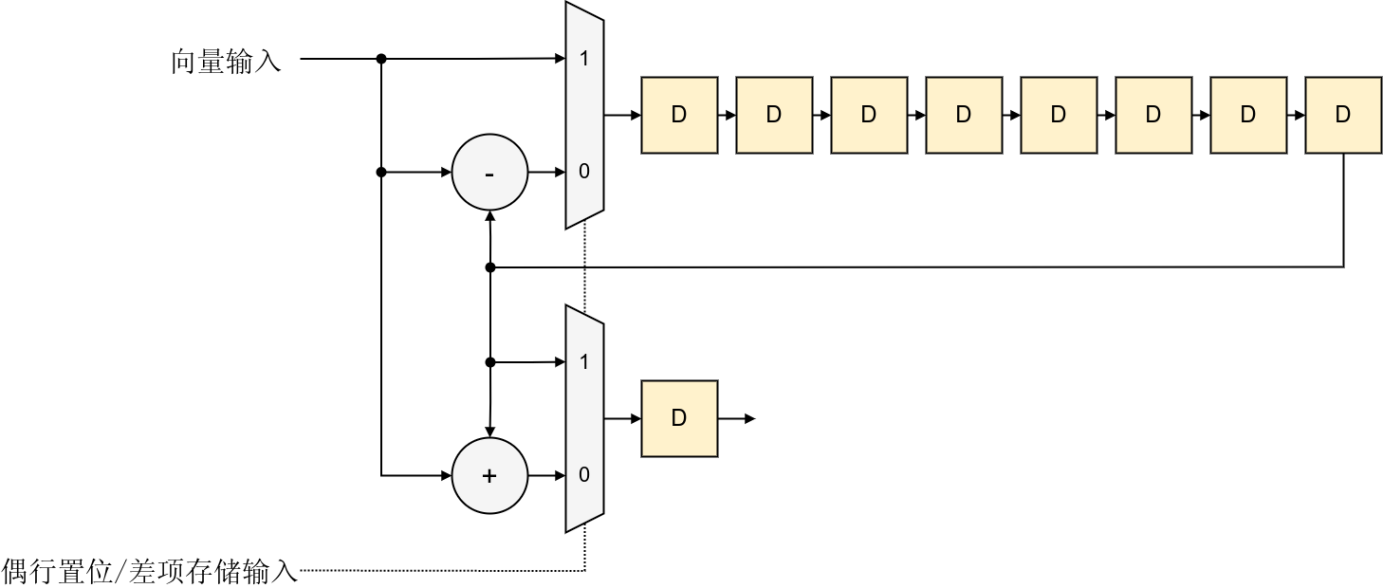
\includegraphics[scale=0.8]{./pictures/和差项生成.png}
        \caption{和差项生成部分}
        \label{和差项生成}
      \end{figure}
      \begin{figure}[H]
        \centering
        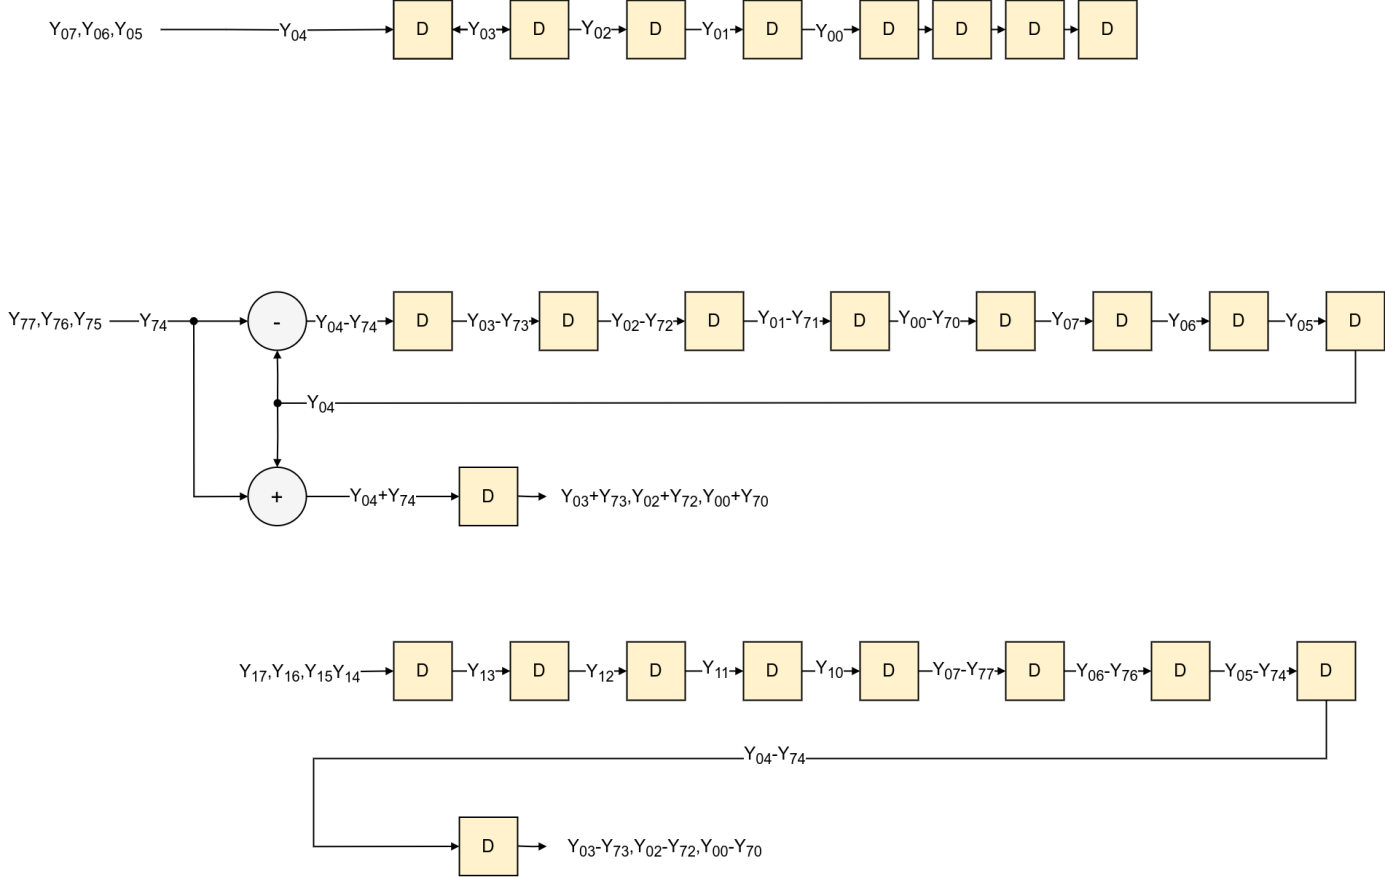
\includegraphics[scale=0.8]{./pictures/和差项生成步骤.png}
        \caption{$Z^{T}$和差项生成步骤}
        \label{和差项生成步骤}
      \end{figure}
      该结构的运行步骤如图所示,当的第1行($Z_{00}$到$Z_{07}$)输入时,偶
      行置位为1。将该行输入到8拍的移位寄存器上;当的第8行($Z_{70}$到$Z_{
      77}$)输入时,偶行置位为0。将移位寄存器输出的1行和8行输入到减法器并
      送回到移位寄存器,同时输入到加法器输出和项;当Y的第2行($Z_{10}$到$
      Z_{17}$)输入时,偶行置位为1将该行输入到8拍的移位寄存器上,同时移位
      寄存器输出上一步骤计算的差项。其他行之间的和差项运算同理。
  \subsection{数据预处理模块}
    \vspace{1em}
  \subsection{熵编码模块}
    \vspace{1em}
  \subsection{JPEG文件格式生成模块}
    \vspace{1em}

\newpage
\section{JPEG编解码系统FPGA实现以及验证}
  \subsection{验证系统模块划分}

\end{spacing}
\end{document}
